\documentclass[12pt]{article}
\usepackage[left=0.5in, right=0.5in, top=0.75in, bottom=0.5in]{geometry}
\usepackage{epsfig,graphics,amsmath,color,multicol,enumitem,tabularx,pbox,url}
\usepackage{cancel}
\usepackage{vwcol} 
%\usepackage[firstpage]{draft watermark}

\setlist{noitemsep}
\setlist{nolistsep}

\pagestyle{empty}

\begin{document}


\begin{tabular*}{\textwidth}{@{\extracolsep{\fill}}l l}
\textbf{Second Derivative}  &  Wizard name: \hrulefill \\
%\textbf{\today} & MATH 157, Hogwart's House: \rule{4cm}{0.5pt}  \\
\textbf{Math 160 } & MATH 160 Hogwart's House:\hspace{2cm} \\
\hline\hline
\end{tabular*} 

\normalsize 

\section*{Motivating Second Derivatives of Functions}
Using the graph of $f(x)$ below, work through the following questions


\begin{minipage}[c]{0.6\linewidth}
    \begin{center}
        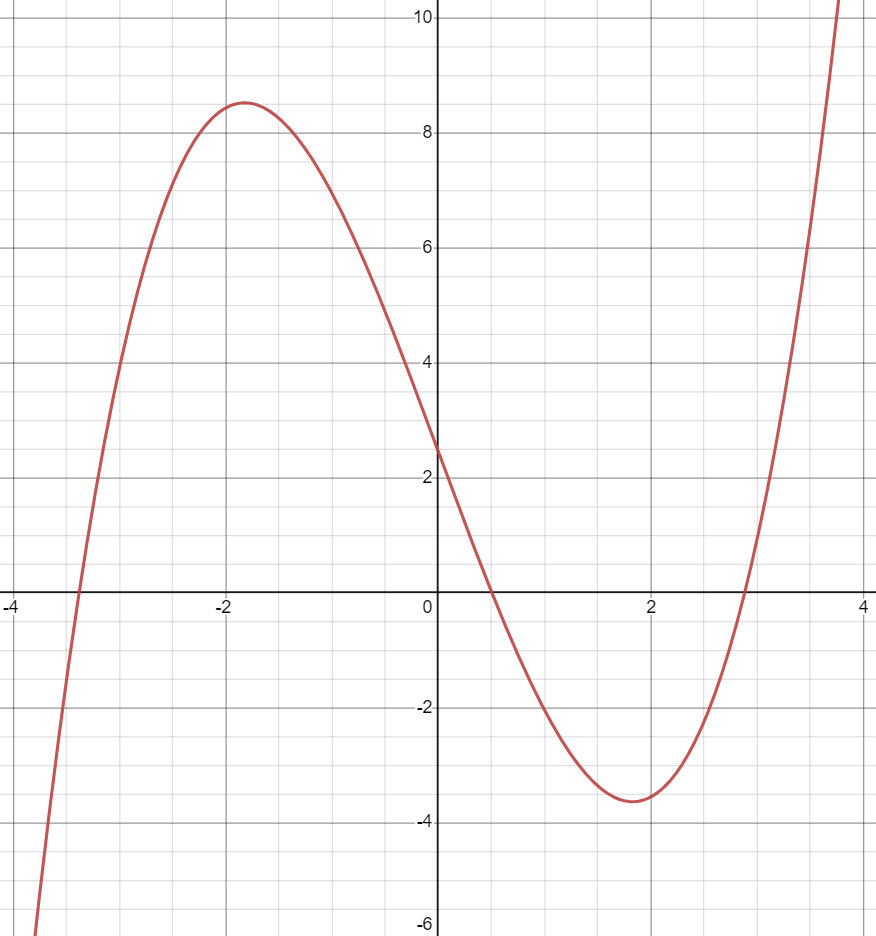
\includegraphics[scale=0.6, trim=0 80 0 50,clip]{cubic.png}
    \end{center}
\end{minipage}
\begin{minipage}[c]{0.4\linewidth}
\begin{itemize}
\item[(a)] When is $f(x)$ increasing (when reading left to right)?\\\\\\
\item[(b)] When is $f(x)$ decreasing?\\\\\\
\item[(c)] When does $f(x)$ change between increasing and decreasing? What are the values of $f'(x)$ at those points? Draw their tangent lines.\\\\\\

\end{itemize}
\end{minipage}
\\

\begin{itemize}
\item[(d)] Draw the tangent lines at $x=-3$, $x=-2$, $x=1.75$, $x=0$. Order $f'(-3)$, $f'(-2)$, $f'(-1.75)$, $f'(0)$ from least to greatest\\\\\\
\item[(e)] Draw the tangent lines at $x=1.75$, $x=2.25$, $x=3$. Order $f'(0)$, $f'(1.75)$, $f'(2.25)$, $f'(3)$ from least to greatest.\\\\\\
\item[(f)] Is $f'(x)$ increasing on $[2,4]$? Justify your reasoning!\\\\\\\\
\item[(g)] Find an interval where $f'(x)$ in decreasing. What does this tell us about the derivative of $f'(x)$? Justify your reasoning!\\\\\\\\
\item[(h)] Find a value of $x$ where $f'(x)$ change from decreasing to increasing? What does this tell us about the derivative of $f'(x)$?
\end{itemize}
\newpage
\section*{Concavity and the Second Derivative}
\begin{itemize}
    \item[(1)] Sketch a function that is always increasing and always concave down \\\\\\
    \item[(2)] Sketch a function that is always increasing and always concave up \\\\\\
    \item[(3)] Compute the following derivatives:
    \begin{itemize}
        \begin{multicols}{2}
        \item[(a)] $\frac{d^2}{dx^2}\left[4x^5\right]$
        \item[(b)] $\frac{d^2}{dx^2}\left[\frac{1}{\sqrt{x}}\right]$
        \end{multicols}
    \end{itemize}
    \vspace{1.5in}
    \item[(4)] Sketch the graph of a function on $[0,8]$ that has all of the following
    \begin{itemize}
        \begin{multicols}{2}
            \item $\displaystyle f'(x)>0$ for $0<x<4$
            \item $\displaystyle f'(x)<0$ for $x>4$
            \item $\displaystyle f''(x)<0$ for $4<x<6$
            \item $\displaystyle f''(x)>0$ for $x>6$
            \item $f(x)$ is continuous on $0\leq x\leq 8$
            \item $f(4)=6$
            \item $f(6)=2$
        \end{multicols}
    \end{itemize}
    \end{itemize}
    \vspace{.25in}
    \begin{center}
        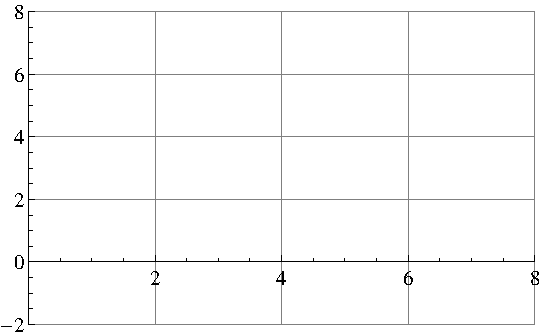
\includegraphics[scale=1.75]{grid.pdf}
    \end{center}

\end{document}
